%# -*- coding: utf-8 -*-
%!TEX encoding = UTF-8 Unicode
%!TEX TS-program = xelatex
% vim:ts=4:sw=4
%
% 以上设定默认使用 XeLaTex 编译,并指定 Unicode 编码,供 TeXShop 自动识别

% Author: Yunhui Fu <yhfudev@gmail.com>
% License: Creative Commons (CC BY 4.0)

\section{\cnt{ICA Style Models}{独立成分分析样式建模}{}}


\subsection{\cnt{Independent Component Analysis}{独立成分分析}{}} \label{chp:indepcomponanalysis}

\subsubsection{\cnt{Introduction}{概述}{}}


\cnt{If you recall, in sparse coding(\ref{chp:sparsecoding}), we wanted to learn an \emph{over-complete} basis for the data. In particular, this implies that the basis vectors that we learn in sparse coding will not be linearly independent. While this may be desirable in certain situations, sometimes we want to learn a linearly independent basis for the data. In independent component analysis (ICA), this is exactly what we want to do. Further, in ICA, we want to learn not just any linearly independent basis, but an \emph{orthonormal} basis for the data. (An orthonormal basis is a basis $(\phi_1, \ldots \phi_n)$ such that $\phi_i \cdot \phi_j = 0$ if $i \ne j$ and 1 if $i = j$).}
    {试着回想一下,在介绍 稀疏编码(\ref{chp:sparsecoding})算法中我们想为样本数据学习得到一个\emph{超完备}基(over-complete basis)。具体来说,这意味着用稀疏编码学习得到的基向量之间不一定线性独立。尽管在某些情况下这已经满足需要,但有时我们仍然希望得到的是一组线性独立基。独立成分分析算法(ICA)正实现了这一点。而且,在 ICA 中,我们希望学习到的基不仅要线性独立,而且还是一组标准\emph{正交}基。(一组标准正交基 $(\phi_1, \ldots \phi_n)$ 需要满足条件:$\phi_i \cdot \phi_j = 0$(如果 $i \ne j$)或者 $\phi_i \cdot \phi_j = 1$(如果 $i = j$))}
    {}

\cnt{Like sparse coding, independent component analysis has a simple mathematical formulation. Given some data $x$, we would like to learn a set of basis vectors which we represent in the columns of a matrix $W$, such that, firstly, as in sparse coding, our features are \emph{sparse}; and secondly, our basis is an \emph{orthonormal} basis. (Note that while in sparse coding, our matrix $A$ was for mapping \emph{features} $s$ to \emph{raw data}, in independent component analysis, our matrix $W$ works in the opposite direction, mapping \emph{raw data} $x$ to \emph{features} instead). This gives us the following objective function:}
    {与稀疏编码算法类似,独立成分分析也有一个简单的数学形式。给定数据 $x$,我们希望学习得到一组基向量 -- 以列向量形式构成的矩阵 $W$,其满足以下特点:首先,与稀疏编码一样,特征是\emph{稀疏}的;其次,基是标准\emph{正交}的(注意,在稀疏编码中,矩阵 $A$ 用于将\emph{特征} $s$ 映射到\emph{原始数据},而在独立成分分析中,矩阵 $W$ 工作的方向相反,是将\emph{原始数据} $x$ 映射到\emph{特征})。这样我们得到以下目标函数:}
    {}

$$
    J(W) = \lVert Wx \rVert_1 
$$

\cnt{This objective function is equivalent to the sparsity penalty on the features $s$ in sparse coding, since $Wx$ is precisely the features that represent the data. Adding in the orthonormality constraint gives us the full optimization problem for independent component analysis:}
    {由于 $Wx$ 实际上是描述样本数据的特征,这个目标函数等价于在稀疏编码中特征 $s$ 的稀疏惩罚项。加入标准正交性约束后,独立成分分析相当于求解如下优化问题: }
    {}
$$
    \begin{array}{rcl} {\rm minimize} & \lVert Wx \rVert_1 \\ {\rm s.t.} & WW^T = I \\ \end{array} 
$$

\cnt{As is usually the case in deep learning, this problem has no simple analytic solution, and to make matters worse, the orthonormality constraint makes it slightly more difficult to optimize for the objective using gradient descent -- every iteration of gradient descent must be followed by a step that maps the new basis back to the space of orthonormal bases (hence enforcing the constraint).}
    {与深度学习中的通常情况一样,这个问题没有简单的解析解,而且更糟糕的是,由于标准正交性约束,使得用梯度下降方法来求解该问题变得更加困难 -- 每次梯度下降迭代之后,必须将新的基映射回正交基空间中(以此保证正交性约束)。}
    {}

\cnt{In practice, optimizing for the objective function while enforcing the orthonormality constraint (as described in Orthonormal ICA \ref{chp:icaorth} section below) is feasible but slow. Hence, the use of orthonormal ICA is limited to situations where it is important to obtain an orthonormal basis (TODO: what situations).}
    {实践中,在最优化目标函数的同时施加正交性约束(如下一节 正交ICA \ref{chp:icaorth} 中讲到的)是可行的,但是速度慢。在标准正交基是不可或缺的情况下,标准正交ICA的使用会受到一些限制。(哪些情况见:TODO ) }
    {}


\subsubsection{\cnt{Orthonormal ICA}{正交ICA}{}} \label{chp:icaorth}


\cnt{The orthonormal ICA objective is:}
    {标准正交ICA的目标函数是: }
    {}

$$
\begin{array}{rcl} {\rm minimize} & \lVert Wx \rVert_1 \\ {\rm s.t.} & WW^T = I \\ \end{array} 
$$

\cnt{Observe that the constraint $WW^T = I$ implies two other constraints.}
    {通过观察可知,约束 $WW^T = I$ 隐含着另外两个约束: }
    {}

\cnt{Firstly, since we are learning an orthonormal basis, the number of basis vectors we learn must be less than the dimension of the input. In particular, this means that we cannot learn over-complete bases as we usually do in sparse coding(\ref{chp:sparsecodingautoencinterp}).}
    {第一,因为要学习到一组标准正交基,所以基向量的个数必须小于输入数据的维度。具体来说,这意味着不能像通常在 稀疏编码中所做的那样来学习得到超完备基(over-complete bases)。 }
    {}

\cnt{Secondly, the data must be ZCA whitened(\ref{chp:whitening}) with no regularization (that is, with $\epsilon$ set to 0). (TODO Why must this be so?)}
    {第二,数据必须经过无正则 ZCA白化(也即,$\epsilon$设为0)。(为什么必须这样做?见TODO) }
    {}

\cnt{Hence, before we even begin to optimize for the orthonormal ICA objective, we must ensure that our data has been whitened, and that we are learning an \emph{under-complete} basis.}
    {因此,在优化标准正交ICA目标函数之前,必须确保数据被白化过,并且学习的是一组\emph{不完备}基(under-complete basis)。 }
    {}

\cnt{Following that, to optimize for the objective, we can use gradient descent, interspersing gradient descent steps with projection steps to enforce the orthonormality constraint. Hence, the procedure will be as follows:}
    {然后,为了优化目标函数,我们可以使用梯度下降法,在梯度下降的每一步中增加投影步骤,以满足标准正交约束。过程如下: }
    {}

\cnt{Repeat until done:}
    {重复以下步骤直到完成: }
    {}

\cnt{$W \leftarrow W - \alpha \nabla_W \lVert Wx \rVert_1$}
    {}
    {}

\cnt{$W \leftarrow \operatorname{proj}_U W$ where $U$ is the space of matrices satisfying $WW^T = I$}
    {$W \leftarrow \operatorname{proj}_U W$, 其中 $U$ 是满足 $WW^T = I$ 的矩阵空间 }
    {}

\cnt{In practice, the learning rate $\alpha$ is varied using a line-search algorithm to speed up the descent, and the projection step is achieved by setting $W \leftarrow (WW^T)^{-\frac{1}{2}} W$, which can actually be seen as ZCA whitening (TODO explain how it is like ZCA whitening).}
    {在实际中,学习速率$\alpha$是可变的,使用一个线搜索算法来加速梯度.投影步骤通过设置 $W \leftarrow (WW^T)^{-\frac{1}{2}} W$ 来完成,这实际上可以看成就是ZCA白化(TODO:解释为什么这就象ZCA白化). }
    {}



\subsubsection{\cnt{Topographic ICA}{拓扑ICA}{}}


\cnt{Just like sparse coding(\ref{chp:sparsecodingautoencinterp}), independent component analysis can be modified to give a topographic variant by adding a topographic cost term.}
    {与 稀疏编码(\ref{chp:sparsecodingautoencinterp})算法类似,加上一个拓扑代价项,独立成分分析法可以修改成具有拓扑性质的算法。 }
    {}



\subsection{\cnt{Exercise:Independent Component Analysis}{}{}}

\cnt{In this exercise, you will implement Independent Component Analysis(\ref{chp:indepcomponanalysis}) on color images from the STL-10 dataset.}
    {}
    {}

\cnt{In the file \href{http://ufldl.stanford.edu/wiki/resources/independent_component_analysis_exercise.zip}{independent\_component\_analysis\_exercise.zip} we have provided some starter code. You should write your code at the places indicated ``YOUR CODE HERE" in the files.}
    {}
    {}

\cnt{For this exercise, you will need to modify \texttt{OrthonormalICACost.m} and \texttt{ICAExercise.m}.}
    {}
    {}


\subsubsection{\cnt{Dependencies}{}{}}

\cnt{You will need:}
    {}
    {}
\begin{itemize}
  \item \cnt{\texttt{computeNumericalGradient.m} from Exercise:Sparse Autoencoder(\ref{chp:execsparseautoenc})}
    {}
    {}

  \item \cnt{\texttt{displayColorNetwork.m} from Exercise:Learning color features with Sparse Autoencoders(\ref{chp:execcolorfeaturesparseautoenc})}
    {}
    {}
\end{itemize}

\cnt{The following additional file is also required for this exercise:}
    {}
    {}
\begin{itemize}
  \item \cnt{\href{http://ufldl.stanford.edu/wiki/resources/stl10_patches_100k.zip}{Sampled $8 \times 8$ patches from the STL-10 dataset (stl10\_patches\_100k.zip)} }
    {}
    {}
\end{itemize}

\emph{
\cnt{If you have not completed the exercises listed above, we strongly suggest you complete them first.
}
    {}
    {}
}


\subsubsection{\cnt{Step 0: Initialization}{}{}}


\cnt{In this step, we initialize some parameters used for the exercise.}
    {}
    {}


\subsubsection{\cnt{Step 1: Sample patches}{}{}}


\cnt{In this step, we load and use a portion of the $8 \times 8$ patches from the STL-10 dataset (which you first saw in the exercise on linear decoders \ref{chp:execcolorfeaturesparseautoenc}).}
    {}
    {}


\subsubsection{\cnt{Step 2: ZCA whiten patches}{}{}}


\cnt{In this step, we ZCA whiten the patches as required by orthonormal ICA.}
    {}
    {}


\subsubsection{\cnt{Step 3: Implement and check ICA cost functions}{}{}}



\cnt{In this step, you should implement the ICA cost function: \texttt{orthonormalICACost} in \texttt{orthonormalICACost.m}, which computes the cost and gradient for the orthonormal ICA objective. Note that the orthonormality constraint is not enforced in the cost function. It will be enforced by a projection in the gradient descent step, which you will have to complete in step 4.}
    {}
    {}

\cnt{When you have implemented the cost function, you should check the gradients numerically.}
    {}
    {}

\cnt{Hint - if you are having difficulties deriving the gradients, you may wish to consult the page on deriving gradients using the backpropagation idea (\ref{chp:derivegradbackpropidea}).}
    {}
    {}


\subsubsection{\cnt{Step 4: Optimization}{}{}}


\cnt{In step 4, you will optimize for the orthonormal ICA objective using gradient descent with backtracking line search (the code for which has already been provided for you. For more details on the backtracking line search, you may wish to consult the appendix(\ref{chp:execicaappendix}) of this exercise). The orthonormality constraint should be enforced with a projection, which you should fill in.}
    {}
    {}

\cnt{Once you have filled in the code for the projection, check that it is correct by using the verification code provided. Once you have verified that your projection is correct, comment out the verification code and run the optimization. 1000 iterations of gradient descent should take less than 15 minutes, and produce a basis which looks like the following:}
    {}
    {}


\begin{figure}[ht] \centering
  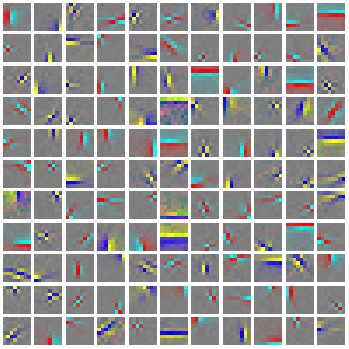
\includegraphics[width=0.4\textwidth]{figures/OrthonormalICAFeatures.png}
  %\caption{}\label{fig:step1}
\end{figure}

\cnt{It is comparatively difficult to optimize for the objective while enforcing the orthonormality constraint using gradient descent, and convergence can be slow. Hence, in situations where an orthonormal basis is not required, other faster methods of learning bases (such as sparse coding \ref{chp:sparsecodingautoencinterp}) may be preferable.}
    {}
    {}


\subsubsection{\cnt{Appendix}{}{}} \label{chp:execicaappendix}



\textbf{\cnt{Backtracking line search}{}{}}


\cnt{The backtracking line search used in the exercise is based off that in Convex Optimization by Boyd and Vandenbergh(\url{http://www.stanford.edu/~boyd/cvxbook/}). In the backtracking line search, given a descent direction $\vec{u}$ (in this exercise we use $\vec{u} = -\nabla f(\vec{x})$), we want to find a good step size t that gives us a steep descent. The general idea is to use a linear approximation (the first order Taylor approximation) to the function f at the current point $\vec{x}$, and to search for a step size t such that we can decrease the function's value by more than $\alpha$ times the decrease predicted by the linear approximation ($\alpha \in (0, 0.5)$. For more details, you may wish to consult the \href{http://www.stanford.edu/~boyd/cvxbook/}{book}.}
    {}
    {}

\cnt{However, it is not necessary to use the backtracking line search here. Gradient descent with a small step size, or backtracking to a step size so that the objective decreases is sufficient for this exercise.}
    {}
    {}



